\documentclass{article}

\usepackage{array}
\usepackage{float}
\usepackage{paracol}
\usepackage{graphicx}
\usepackage{hyperref}
\usepackage{xcolor}
\usepackage[spanish]{babel}
\usepackage[a4paper, total={7in, 10in}]{geometry}

\usepackage[backend=biber,style=ieee]{biblatex}
\addbibresource{biblio.bib}


\title{Clasificación No Supervisada}
\author{Marco Ciccalè Baztán}
\date{10/05/2024}

\begin{document}

\begin{center}
\rule{\textwidth}{1pt}
{\huge \begin{center}\textbf{Clasificación No Supervisada}\end{center}}
\vspace*{.5cm}
{\LARGE Marco Ciccalè Baztán}
\rule{\textwidth}{1pt}
\end{center}

\section{Introducción}

\noindent En este documento de detallará con exhaustividad todo el proceso que se ha seguido para abordar un problema de clasificación no supervisada.
Para resolver este problema, se ha decidido experimentar con 3 algoritmos de aprendizaje no supervisado pertenecientes a diferentes familias de \textit{clustering}:
\textit{KMeans} (\textit{clustering} particional),
\textit{Agglomerative} (\textit{clustering} jerárquico) y
\textit{Gaussian Mixture Models} (\textit{clustering} probabilístico).
El objetivo de este experimento es evaluar e interpretar cómo se comportan los diferentes algoritmos ante este problema.

\section{Descripción del problema}

\noindent El problema que se aborda en este experimento nace de una base de datos con información de un conjunto de 167 países alrededor del mundo en diferentes continentes.
Dado este conjunto de datos, se busca agrupar los países en diferentes grupos para poder evaluar cuáles de ellos pueden necesitar ayuda humanitaria con más urgencia.

\section{Metodología}

\subsection{Conjunto de Datos}

\noindent El conjunto de datos que se ha usado para este experimento fue extraído de la plataforma \textit{Kaggle} \cite{dataset}.
El tamaño del dataset son 167 filas y 10 columnas,
cada fila del conjunto de datos corresponde a un país, y cada columna un valor de las siguientes medidas:

\begin{itemize}
  \item \verb|country|: El nombre del país (nominal).
  \item \verb|child_mort|: Cantidad de muertes de niños menores de 5 años por cada 1000 nacimientos (continua).
  \item \verb|exports|: Exportación de bienes per cápita (continua).
  \item \verb|health|: Cantidad de recursos invertidos en salud per cápita (continua).
  \item \verb|imports|: Importación de bienes per cápita (continua).
  \item \verb|income|: Ingresos per cápita (continua).
  \item \verb|inflation|: La inflación anual (continua).
  \item \verb|life_expec|: La media de años de vida estimados (continua).
  \item \verb|total_fer|: La media de niños que nacen por cada mujer (continua).
  \item \verb|gdpp|: PIB per cápita (continua).
\end{itemize}

\subsection{Preprocesado de los datos}

\noindent Dada la naturaleza de los algoritmos de \textit{clustering}, las variables no númericas en la mayoría de los casos no suponen una información relevante para el algoritmo.
En este caso, el nombre del país es absolutamente irrelevante para los algoritmos.
Por ello, se eliminó del conjunto de datos para los experimentos, aunque posteriormente fue útil para determinar los países que pertenecen a cada grupo.\\

\noindent Por otro lado, en el conjunto de datos, cada variable tiene un rango de valores completamente distinto.
Esta característica afecta directamente a los resultados de los experimentos, ya que una variable con una magnitud en milares sería mucho más discriminante que una variable con una magnitud de unidades.
Para solventar este problema, se utilizó la técnica \verb|MaxAbsScaler| de \textbf{scikit-learn} \cite{sklearn_api},
transformando los valores de cada variable a una misma escala (entre 0 y 1).
Pudiendo así mantener la distribución original de cada variable a la vez que igualar el peso de cada variable en los experimentos.

\subsection{Pruebas realizadas}

\subsubsection{Determinar el número de clusters óptimo de cada modelo}
\label{sec:pasos-individuales}

\noindent Para evaluar el comportamiento de \textit{KMeans} para este problema, se siguieron los siguientes pasos:

\begin{enumerate}
  \item Entrenar distintos modelos de \textit{KMeans} con [2, 5] \textit{clusters} utilizando la distancia euclídea.
  \item Calcular las medias de los coeficientes de \textit{silhouette} para cada uno de los 4 modelos.
  \item Seleccionar el modelo con mayor media de coeficiente de \textit{silhouette}.
  \item Graficar los coeficientes de \textit{silhouette} de cada cluster.
\end{enumerate}

\noindent Para evaluar el comportamiento de \textit{Agglomerative Clustering} para este problema, se siguieron los siguientes pasos:

\begin{enumerate}
  \item Graficar el dendograma del conjunto de datos utilizando la distancia euclídea y el método \textit{ward}.
  \item Elegir el número de \textit{clusters} óptimo dado el dendograma.
  \item Seleccionar el modelo con mayor media de coeficiente de \textit{silhouette}.
\end{enumerate}

\noindent Para evaluar el comportamiento de \textit{Gaussian Mixtures} para este problema, se siguieron los siguientes pasos:

\begin{enumerate}
  \item Entrenar distintos modelos de \textit{Gaussian Mixture} con [2, 8] \textit{clusters} y obtener el \textit{BIC} de cada modelo.
  \item Graficar el \textit{BIC} de cada modelo y seleccionar el número de \textit{clusters} que minimiza el \textit{BIC}
  \item Seleccionar el modelo con mayor media de coeficiente de \textit{silhouette}.
\end{enumerate}

\subsubsection{Mostrar los resultados de los modelos óptimos}

\noindent Los pasos comunes después de haber obtenido el número de \textit{clusters} óptimo para cada algoritmo son los siguientes:

\begin{enumerate}
  \item Graficar la distribución de las 9 variables del conjunto de datos para cada \textit{cluster}.
  \item Graficar un mapa del mundo donde se muestra qué países pertenecen a cada \textit{cluster}.
\end{enumerate}

\section{Resultados}

\subsection{KMeans (Clustering Particional)}
\label{sec:kmeans}

\noindent Después de seguir los pasos detallados en la sección \ref{sec:pasos-individuales}, el número de \textit{clusters} óptimo (modelo que no tiene valores negativos en sus coeficientes de \textit{silhouette} y que maximiza su media) es 2.
La media de los coeficientes de \textit{silhouette} del modelo con 2 \textit{clusters} es \verb|0.329|.
La figura \ref{fig:silhouette} refleja los coeficientes de \textit{silhouette} de cada \textit{cluster} y la media de los coeficientes.

\begin{figure}[H]
  \centering
  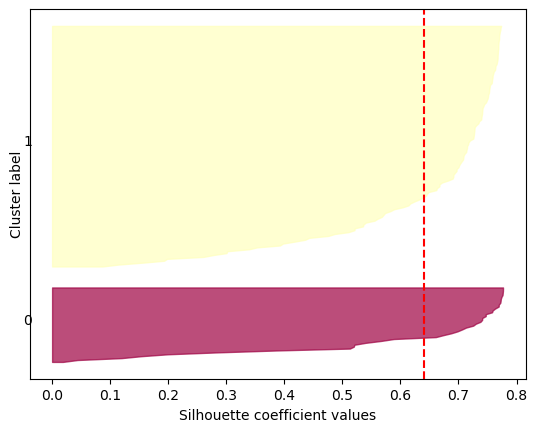
\includegraphics[width=0.5\linewidth]{../images/kmeans/silhouette.png}
  \caption{Coeficientes de \textit{silhouette} para el número de \textit{clusters} óptimo}
  \label{fig:silhouette}
\end{figure}

\columnratio{0.2}
\begin{paracol}{2}
  \sloppy
  \switchcolumn[0]*
  \noindent Por otro lado, en la figura \ref{fig:kmeans-features} se pueden observar las diferencias entre los \textit{clusters} para cada variable.
  Lo más destacable es la diferencia entre las muertes infantiles, la cantidad de ingresos, la fertilidad y el PIB per cápita.
  Observando con detalle estas variables, se puede deducir que el \textit{cluster} 0 seguramente englobe países en vías de desarrollo o subdesarrollados, ya que el PIB per cápita se concentra en un rango de valores muy pequeño y cerca de 0, al igual que los ingresos.
  Además, el número de muertes infantiles y la fertilidad parecen mucho mayores en el \textit{cluster} 0, características que suelen ser atribuídas a países pertenecientes a estos grupos.\\

  \noindent La figura \ref{fig:kmeans-map} representa un mapa del mundo donde se muestra qué países pertenecen a cada cluster.

  \switchcolumn
  \begin{figure}[H]
    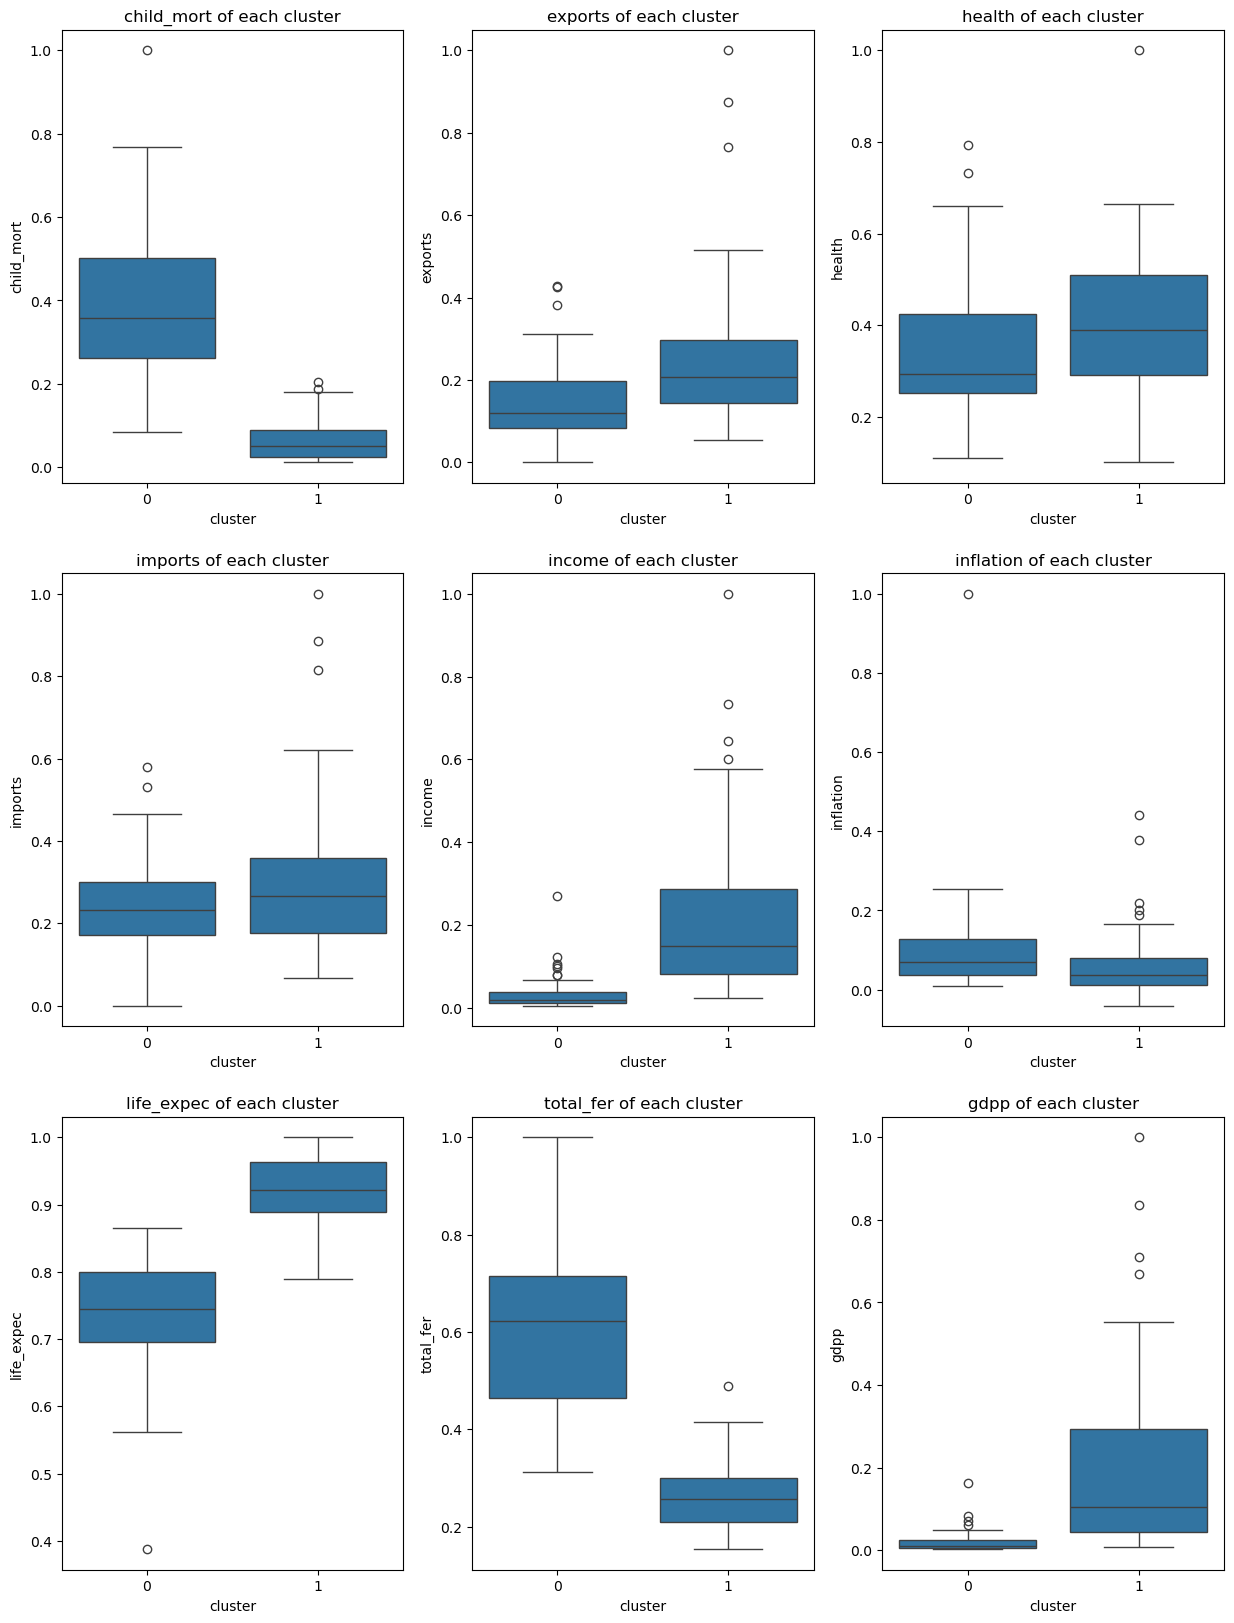
\includegraphics[width=\linewidth]{../images/kmeans/features-dist.png}
    \caption{Distribución de las variables para cada \textit{cluster} en \textit{kmeans}}
    \label{fig:kmeans-features}
  \end{figure}
\end{paracol}

\vspace{-10pt}

\begin{figure}[H]
  \centering
  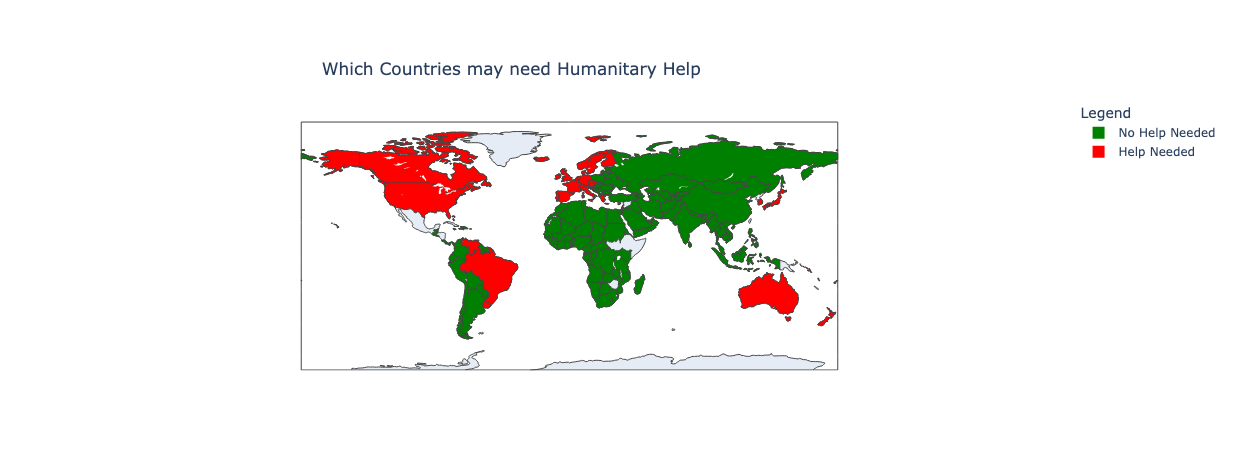
\includegraphics[width=\linewidth]{../images/kmeans/map.png}
  \caption{Distribución de las variables para cada \textit{cluster}}
  \label{fig:kmeans-map}
\end{figure}

\subsection{Agglomerative Clustering (Clustering Jerárquico)}
\noindent Después de seguir los pasos detallados en la sección \ref{sec:pasos-individuales}, se puede identificar en el dendograma de la figura \ref{fig:dendogram} que el número de \textit{clusters} óptimo es 2,
ya que es donde se puede aprecuar una distancia en el eje \textit{y} más notoria entre las dos primeras ramas.

\begin{figure}[H]
  \centering
  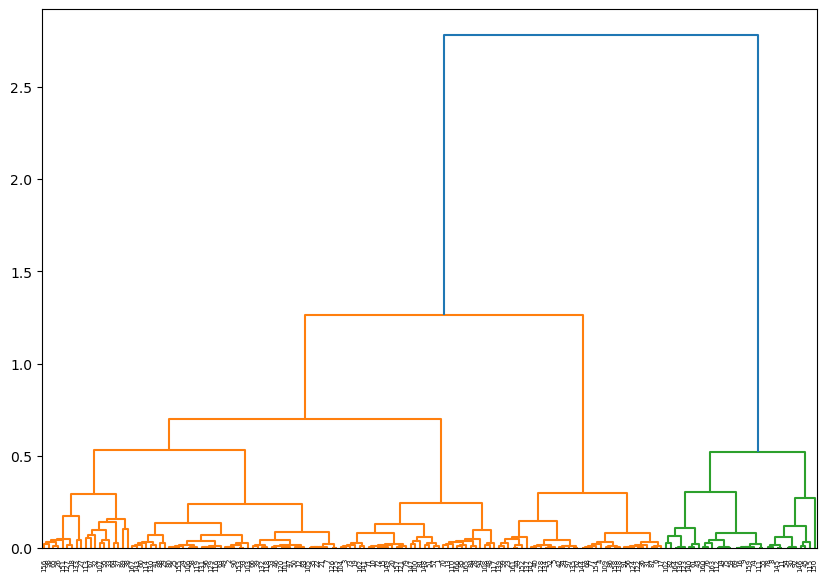
\includegraphics[width=0.4\linewidth]{../images/agglomerative/dendogram.png}
  \caption{Dendograma del conjunto de datos}
  \label{fig:dendogram}
\end{figure}

\noindent Por otro lado, en la figura \ref{fig:agglomerative-features} se puede observar que la diferencias entre los \textit{clusters} para cada variable son prácticamente idénticas al caso anterior de \textit{KMeans} en la sección \ref{sec:kmeans}, seguramente debido a que se está utilizando la distancia euclídea en ambos algoritmos como medida de distancia entre instancias, por lo que las conclusiones obtenidas con \textit{KMeans} son perfectamente válidas para este caso también. 
Esta similitud entre los algoritmos también se puede observar en la figura \ref{fig:agglomerative-map}, ya que también son prácticamente idénticos.

\begin{figure}[H]
  \centering
  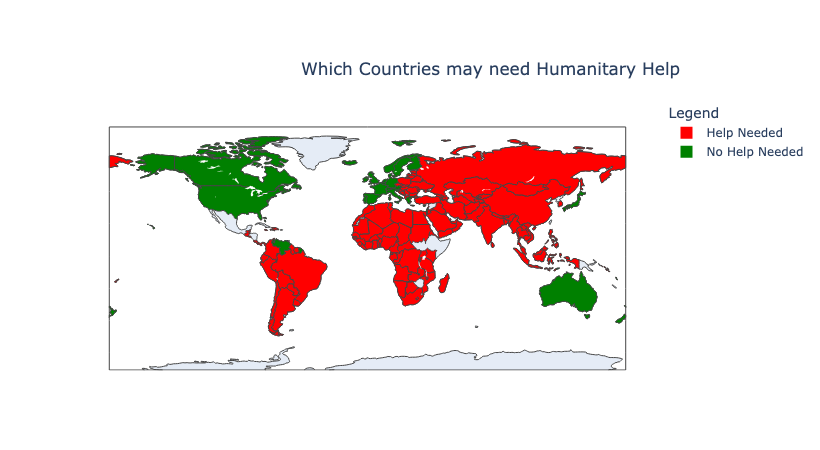
\includegraphics[width=\linewidth]{../images/agglomerative/map.png}
  \caption{Países pertenecientes a cada \textit{cluster}}
  \label{fig:agglomerative-map}
\end{figure}

\subsection{Gaussian Mixture (Clustering Probabilístico)}
\noindent Después de seguir los pasos detallados en la sección \ref{sec:pasos-individuales}, se puede identificar en la figura \ref{fig:bic} que el número de \textit{clusters} que minimiza el \textit{BIC} es 3,
siendo así el número óptimo de \textit{clusters}.

\begin{figure}[H]
  \centering
  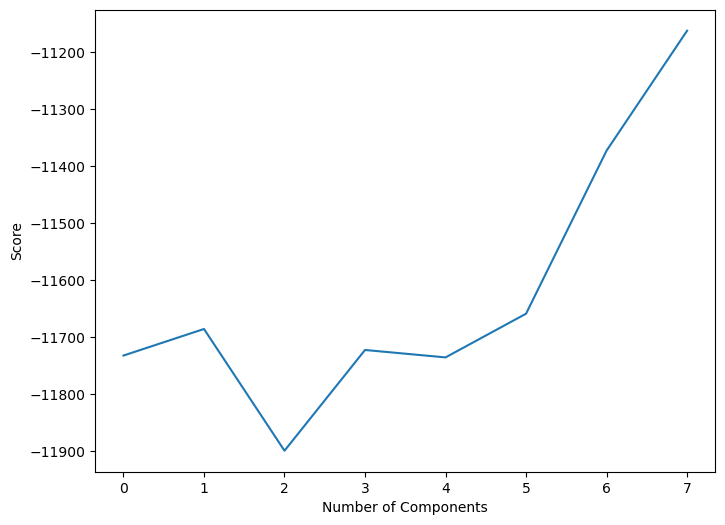
\includegraphics[width=0.35\linewidth]{../images/gaussian/bic.png}
  \caption{Gráfica que representa los valores \textit{BIC} asociados a cada modelo con diferente número de \textit{clusters}}
  \label{fig:bic}
\end{figure}

\columnratio{0.2}
\begin{paracol}{2}
  \sloppy
  \switchcolumn[0]*
  \noindent Por otro lado, en la figura \ref{fig:gaussian-features} se pueden observar las diferencias entre los \textit{clusters} para cada variable.
  Lo más destacable de esta figura es que se pueden observar dos \textit{clusters} (0 y 1) que comparten muchos rasgos sociales como la fertilidad más baja, la esperanza de vida más alta y la baja mortalidad infantil.
  Sin embargo, en rasgos más economicos, pareciera que el \textit{cluster} 0 no está todavía en los niveles en los que está el \textit{cluster} 1,
  como por ejemplo en el PIB per cápita, los ingresos y el gasto en salud.
  De estas conclusiones, se puede deducir que el \textit{cluster} 2 representa a los países en desarrollo total,
  el \textit{cluster} 0 representa a los países que están desarrollados al nivel del \textit{cluster} 1 en temas sociales pero que todavía están atrás en temas económicos,
  y el \textit{cluster} 1 representa a los países desarrollados.

  \noindent La figura \ref{fig:gaussian-map} representa un mapa del mundo donde se muestra qué países pertenecen a cada cluster.

  \switchcolumn
  \begin{figure}[H]
    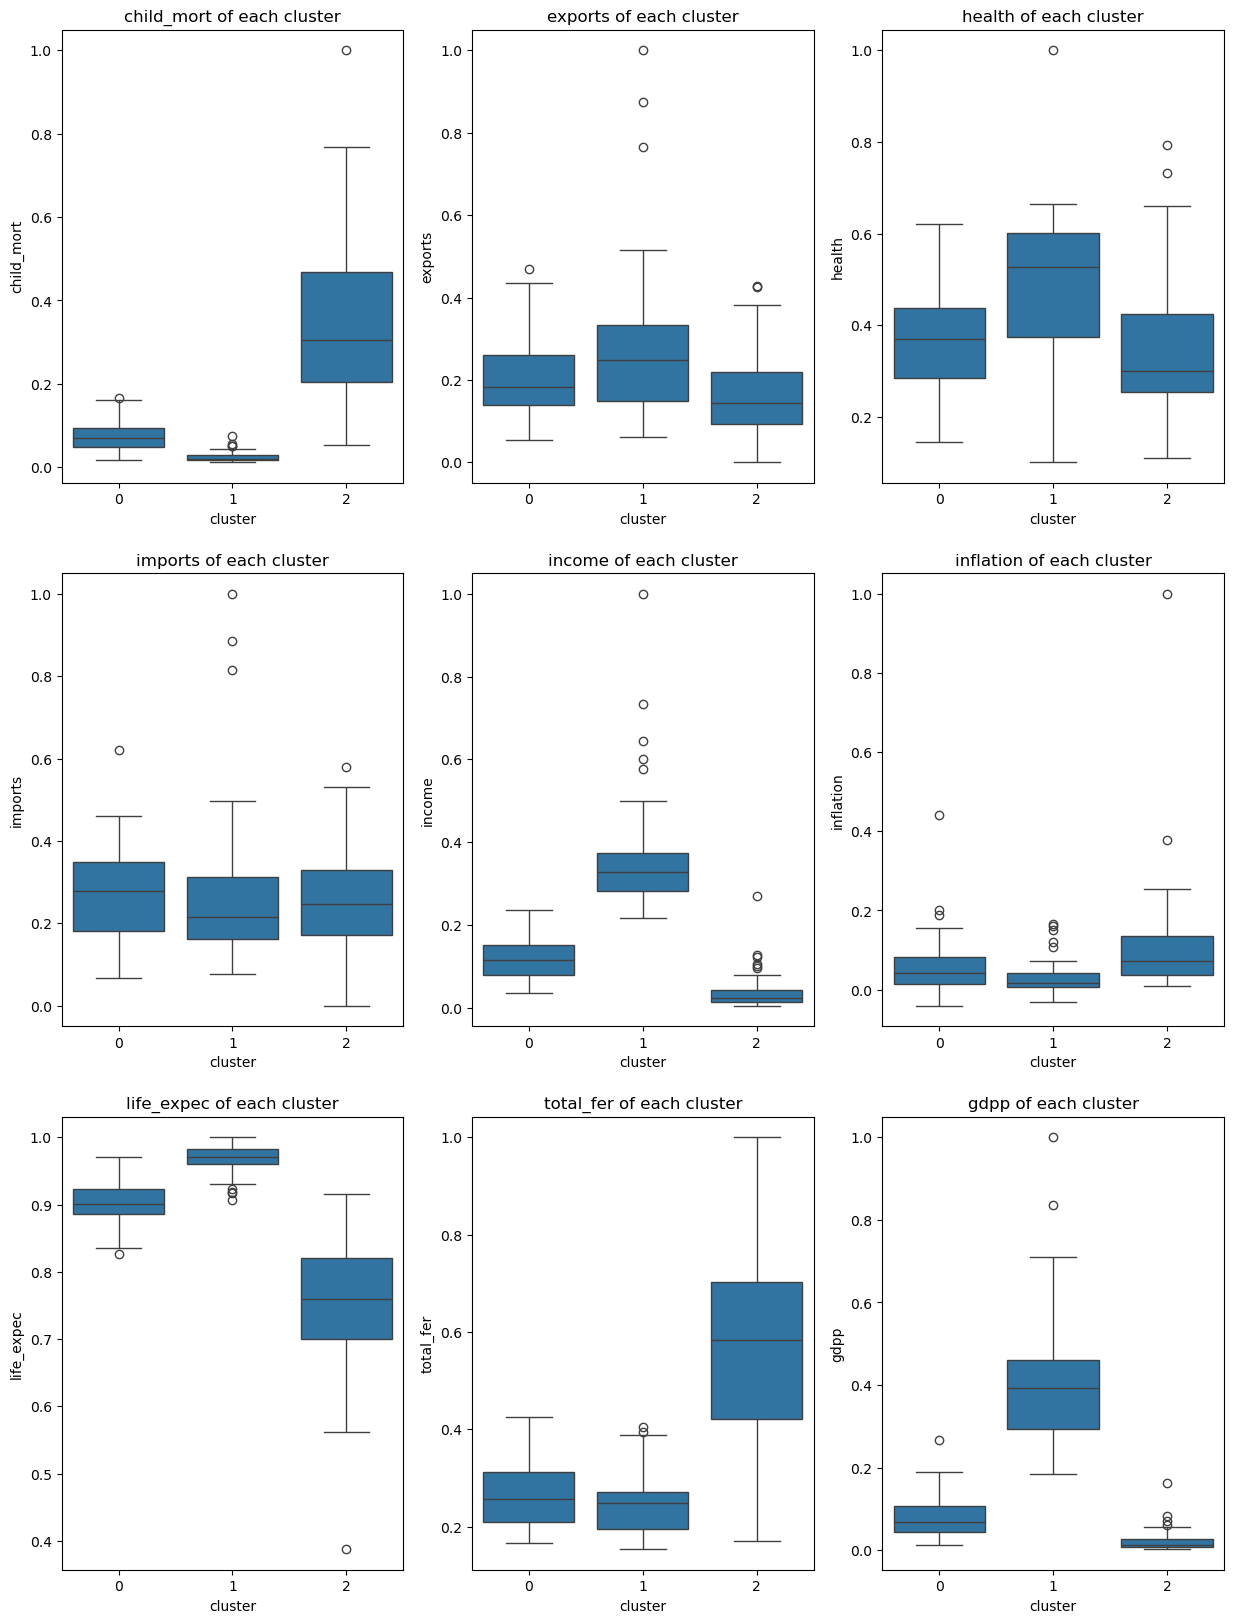
\includegraphics[width=\linewidth]{../images/gaussian/features-dist.png}
    \caption{Distribución de las variables para cada \textit{cluster} en \textit{gaussian mixture}}
    \label{fig:gaussian-features}
  \end{figure}
\end{paracol}

\begin{figure}[H]
  \centering
  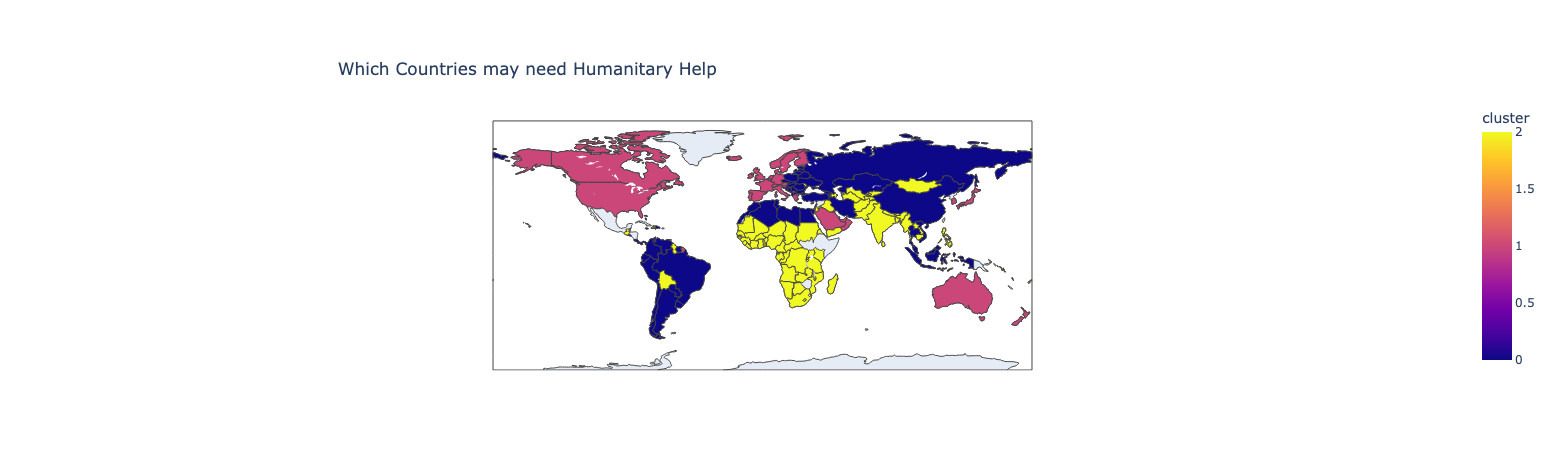
\includegraphics[width=\linewidth]{../images/gaussian/map.png}
  \caption{Países pertenecientes a cada \textit{cluster}}
  \label{fig:gaussian-map}
\end{figure}

\section{Conclusiones}

\noindent Después de haber realizado este experimento, se puede concluir que los algoritmos \textit{KMeans} y \textit{Agglomerative Clustering} a pesar de haber podido distinguir dos posibles grupos, la agrupación no parece muy acertada, ya que identifica países como China y Rusia como parte del \textit{cluster} donde se encuentran países verdaderamente subdesarollados como Sudán.
Esto también se ve reflejado formalmente en el bajo coeficiente de \textit{silhouette} que se muestra en la figura \ref{fig:silhouette} y la distancia no tan pronunciada entre las ramas del dendograma de la figura \ref{fig:dendogram}.\\

\noindent Por otro lado, el algoritmo \textit{Gaussian Mixture} ha podido diferenciar con mayor precisión 3 \textit{clusters} distintos, donde ha agrupado países desarrollados (españa, alemania...), países en vías de desarrollo (rusia, china...) y países subdesarrollados (nigeria, mali). \\

\noindent Una vez realizado este análisis sobre los resultados de los experimentos, se ha podido comprobar formalmente con diferentes técnicas qué países son los que más necesitan ayuda humanitaria, pudiendo así evaluar cómo distribuir las ayudas más eficientemente e intentando ver qué países pueden necesitarla aunque se piense que son países con un nivel de desarrollo más alto.

\addcontentsline{toc}{chapter}{Bibliography}
\printbibliography

\section*{Anexo}

\begin{figure}[H]
  \centering
  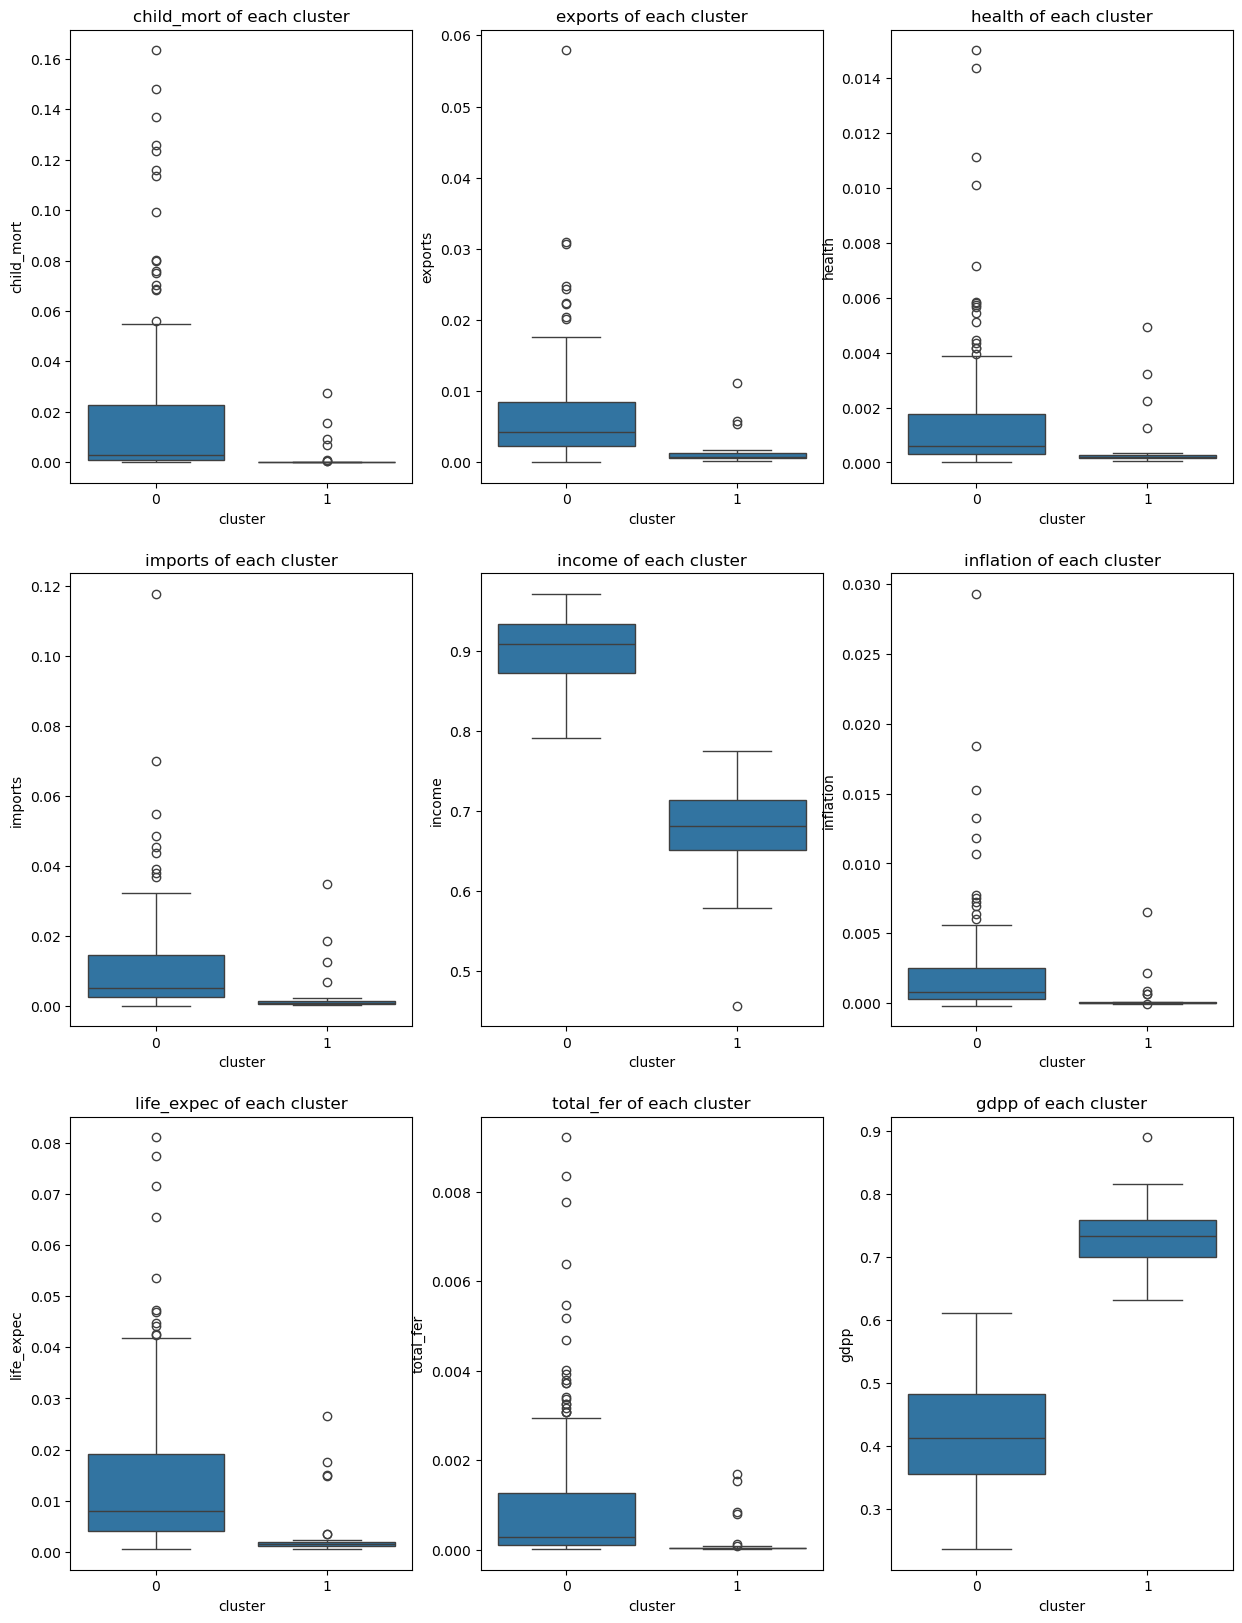
\includegraphics[width=\linewidth]{../images/agglomerative/features-dist.png}
  \caption{Distribución de las variables para cada \textit{cluster} en \textit{agglomerative clustering}}
  \label{fig:agglomerative-features}
\end{figure}

\end{document}
